% This is "sig-alternate.tex" V2.1 April 2013
% This file should be compiled with V2.5 of "sig-alternate.cls" May 2012
%
% This example file demonstrates the use of the 'sig-alternate.cls'
% V2.5 LaTeX2e document class file. It is for those submitting
% articles to ACM Conference Proceedings WHO DO NOT WISH TO
% STRICTLY ADHERE TO THE SIGS (PUBS-BOARD-ENDORSED) STYLE.
% The 'sig-alternate.cls' file will produce a similar-looking,
% albeit, 'tighter' paper resulting in, invariably, fewer pages.
%
% ----------------------------------------------------------------------------------------------------------------
% This .tex file (and associated .cls V2.5) produces:
%       1) The Permission Statement
%       2) The Conference (location) Info information
%       3) The Copyright Line with ACM data
%       4) NO page numbers
%
% as against the acm_proc_article-sp.cls file which
% DOES NOT produce 1) thru' 3) above.
%
% Using 'sig-alternate.cls' you have control, however, from within
% the source .tex file, over both the CopyrightYear
% (defaulted to 200X) and the ACM Copyright Data
% (defaulted to X-XXXXX-XX-X/XX/XX).
% e.g.
% \CopyrightYear{2007} will cause 2007 to appear in the copyright line.
% \crdata{0-12345-67-8/90/12} will cause 0-12345-67-8/90/12 to appear in the copyright line.
%
% ---------------------------------------------------------------------------------------------------------------
% This .tex source is an example which *does* use
% the .bib file (from which the .bbl file % is produced).
% REMEMBER HOWEVER: After having produced the .bbl file,
% and prior to final submission, you *NEED* to 'insert'
% your .bbl file into your source .tex file so as to provide
% ONE 'self-contained' source file.
%
% ================= IF YOU HAVE QUESTIONS =======================
% Questions regarding the SIGS styles, SIGS policies and
% procedures, Conferences etc. should be sent to
% Adrienne Griscti (griscti@acm.org)
%
% Technical questions _only_ to
% Gerald Murray (murray@hq.acm.org)
% ===============================================================
%
% For tracking purposes - this is V2.0 - May 2012

\documentclass{sig-alternate-05-2015}
\usepackage{hyperref}
\usepackage{float}

\begin{document}

% Copyright
\setcopyright{acmcopyright}
%\setcopyright{acmlicensed}
%\setcopyright{rightsretained}
%\setcopyright{usgov}
%\setcopyright{usgovmixed}
%\setcopyright{cagov}
%\setcopyright{cagovmixed}


% DOI
\doi{10.475/133_7}

% ISBN
\isbn{0000-42-1337}

%Conference
\conferenceinfo{Life '16}{May 25, 2016, DK}

\acmPrice{\$15.00}

%
% --- Author Metadata here ---
\conferenceinfo{DIKU}{'16 El Diku, Copenhagen}




\title{Http Server}
\subtitle{[Ugeopgave 2]
\titlenote{}}
%
% You need the command \numberofauthors to handle the 'placement
% and alignment' of the authors beneath the title.
%
% For aesthetic reasons, we recommend 'three authors at a time'
% i.e. three 'name/affiliation blocks' be placed beneath the title.
%
% NOTE: You are NOT restricted in how many 'rows' of
% "name/affiliations" may appear. We just ask that you restrict
% the number of 'columns' to three.
%
% Because of the available 'opening page real-estate'
% we ask you to refrain from putting more than six authors
% (two rows with three columns) beneath the article title.
% More than six makes the first-page appear very cluttered indeed.
%
% Use the \alignauthor commands to handle the names
% and affiliations for an 'aesthetic maximum' of six authors.
% Add names, affiliations, addresses for
% the seventh etc. author(s) as the argument for the
% \additionalauthors command.
% These 'additional authors' will be output/set for you
% without further effort on your part as the last section in
% the body of your article BEFORE References or any Appendices.

\numberofauthors{1} %  in this sample file, there are a *total*
% of EIGHT authors. SIX appear on the 'first-page' (for formatting
% reasons) and the remaining two appear in the \additionalauthors section.
%
\author{
% You can go ahead and credit any number of authors here,
% e.g. one 'row of three' or two rows (consisting of one row of three
% and a second row of one, two or three).
%
% The command \alignauthor (no curly braces needed) should
% precede each author name, affiliation/snail-mail address and
% e-mail address. Additionally, tag each line of
% affiliation/address with \affaddr, and tag the
% e-mail address with \email.
%
% 1st. author
\alignauthor
Mirza Hasanbasic
}
% There's nothing stopping you putting the seventh, eighth, etc.
% author on the opening page (as the 'third row') but we ask,
% for aesthetic reasons that you place these 'additional authors'
% in the \additional authors block, viz.

% Just remember to make sure that the TOTAL number of authors
% is the number that will appear on the first page PLUS the
% number that will appear in the \additionalauthors section.

\maketitle
\begin{abstract}
In this assignment we will be looking at how to implement a simple HTTP server, that will have a subset of the entire HTTP protocol. The HTTP server will still be able to communicate with client and can get multiple connections because of thread implementation. There will be performance and validation discussion about the HTTP server as well as the limitations and testing of the server.
\end{abstract}


%
% The code below should be generated by the tool at
% http://dl.acm.org/ccs.cfm
% Please copy and paste the code instead of the example below.
%
\begin{CCSXML}
<ccs2012>
 <concept>
  <concept_id>10010520.10010553.10010562</concept_id>
  <concept_desc>Computer systems organization~Embedded systems</concept_desc>
  <concept_significance>500</concept_significance>
 </concept>
 <concept>
  <concept_id>10010520.10010575.10010755</concept_id>
  <concept_desc>Computer systems organization~Redundancy</concept_desc>
  <concept_significance>300</concept_significance>
 </concept>
 <concept>
  <concept_id>10010520.10010553.10010554</concept_id>
  <concept_desc>Computer systems organization~Robotics</concept_desc>
  <concept_significance>100</concept_significance>
 </concept>
 <concept>
  <concept_id>10003033.10003083.10003095</concept_id>
  <concept_desc>Networks~Network reliability</concept_desc>
  <concept_significance>100</concept_significance>
 </concept>
</ccs2012>
\end{CCSXML}

\ccsdesc[500]{Computer systems organization~Embedded systems}
\ccsdesc[300]{Computer systems organization~Redundancy}
\ccsdesc{Computer systems organization~Robotics}
\ccsdesc[100]{Networks~Network reliability}


%
% End generated code
%

%
%  Use this command to print the description
%


% We no longer use \terms command
%\terms{Theory}


\section{The Server}
The pseudo coding part was made in collaboration with Mads and Mathias

The server is written in Python and to run it you have to type \texttt{./Server.py} and let the console window be. Now open a new console window and try to connect to the server. The default port is 5000 if this port doesn't work on your computer you may have to change it in the code on line 61.

You can use my \texttt{HTTPClient} to test the server or use telnet or use your own implantation. 

The libraries and frameworks I use are threading, socketServer, os.path, unittest and email.utils when we use the function formatdata. I also have imported serverResponse, parseRequest and returnFile into the \texttt{Server.py} file.

The way the server work, is that it inherit from the ThreadingMixInto create a threaded connection behavior. This class defines the daemon\_threads attribute that tells the server whether it should wait for a thread termination or not. The value is False per default, which means that Python will not exit until the threads that are created by the class have exited. We have set the value to True so for every request a thread is spawned and when the request ends the thread is killed.

It is important to note that the mix in class first as it overrides a method that is defined it TCPServer.

So this means that the server is supporting multiple connections from clients that request some files or something else from the server.

To be able to follow the HTTP standard then the server has a help function to parse the request. Here I have my \texttt{parseReqToDict}. This function will check if the request line is as follows: \texttt{Method SP Request-URI SP HTTP-Version CRLF}. So first it checks for the length of the request line and if it is different than 3 then an error is returned. If the request line is right, then if the requested method is supported if not then it throws a 400 error after that it checks for the separators.
The way we split the data follows the \texttt{JSON} standard for an pleasant readability.
Furthermore if the request is \texttt{HTTP/1.1} then it is required to give a \texttt{HOST} if there is non then error 400 is return

For now the only method that is supported is \texttt{GET} and the headers that are supported are \texttt{host} and \texttt{connection}
These headers are the simplest and the most necessary headers to support. 

The reason I support the Host request-header is that it specifies the host and port number of the resource that is requested. It is also required that a client must include a Host header field in all HTTP/1.1 request messages and all internet based HTTP/1.1 servers must respond with a 400 (Bad request) status code to any HTTP/1.1 request messages which lacks the Host header field.

The other header i.e. the connection allows the sender to specify options that are desired for that particular connection. Also HTTP/1.1 must parse the connection header field before a message is forwarded and connection options are signaled by the presence of a connection token in the connection header field. The HTTP/1.1 defines the "close" connection option for the sender to signal that the connection will be closed after completion of the response. It is also notable that HTTP/1.1 apllication that do not support persistent connection must include the "close" connection option in every message. The connection also protects from a mistaken forwarding.

For the response part of the server, we need to have a correct response. For this I use the \texttt{serverResponse}. I have a response template that tells how a response will be as output. First I check if the given method a client request is supported by the server if not then I return 405 as in method not allowed. Hereafter I check for the filecontent i.e. the \texttt{abs\_path} if you only look for the localhost then it will return a list of the files in the client folder. When the filecontent has passed the \texttt{200 OK} is return back to the client. If everything fails then the client will get a 400 error as bad request.


\subsection{Code structure}
I use 4 files. The 4 files are \texttt{Server.py}, \texttt{serverResponse.py}, \texttt{parseReqToDict.py} and \texttt{returnFile.py}. The only that handles the server i.e. creates it and the needed threads is the \texttt{Server.py} file and this file uses the other 3 as helper files to be sure that the parsed request is correct, that crafted response follows the HTTP RFC.

\subsection{Performance and validation}
The performance of the server is fine as the validation of the hash checksum seems to match the zip files I tested it on. Since the sums are MD5 I used \texttt{md5sum filename} and the md5sums can be seen in the appendix as well as the place where I downloaded the files from.

\subsection{Limitations}
The only limitation I could find and test was that the server timeouts when it gets a request from two or more clients that request a file larger than 512MB. The error I got was from the socketServer framework and no matter if I made the BUFFER\_SIZE bigger it wouldn't work with a bigger file than 512MB for two or more clients that made a request to the server

The only method that the server can handle is the GET method and it only supports two headers i.e. host and connection

\subsection{Testing}
The way I tested the server was that in one console I initiated the server. Then I opened two more consoles and tried to download a file from the server simultaneously. This seemed to work fine, both my HTTPClients recieved a Status code 200 OK: Connection to 127.0.0.1 successful and that the response was written to the filename I have given.
I chose to download a 512MB file as explained in the subsection Performance and validation. Hereafter I checked the checksum (md5sum) for both the files and they matched. This was done in the console window.

I have some unittesting in the file \texttt{parseReqToDict} to test whether it parses the request correctly and is it seems that unittest returns that everything is as expected.

\newpage
\onecolumn
%APPENDICES are optional
%\balancecolumns
\appendix
%Appendix A
\section{Unittesting}
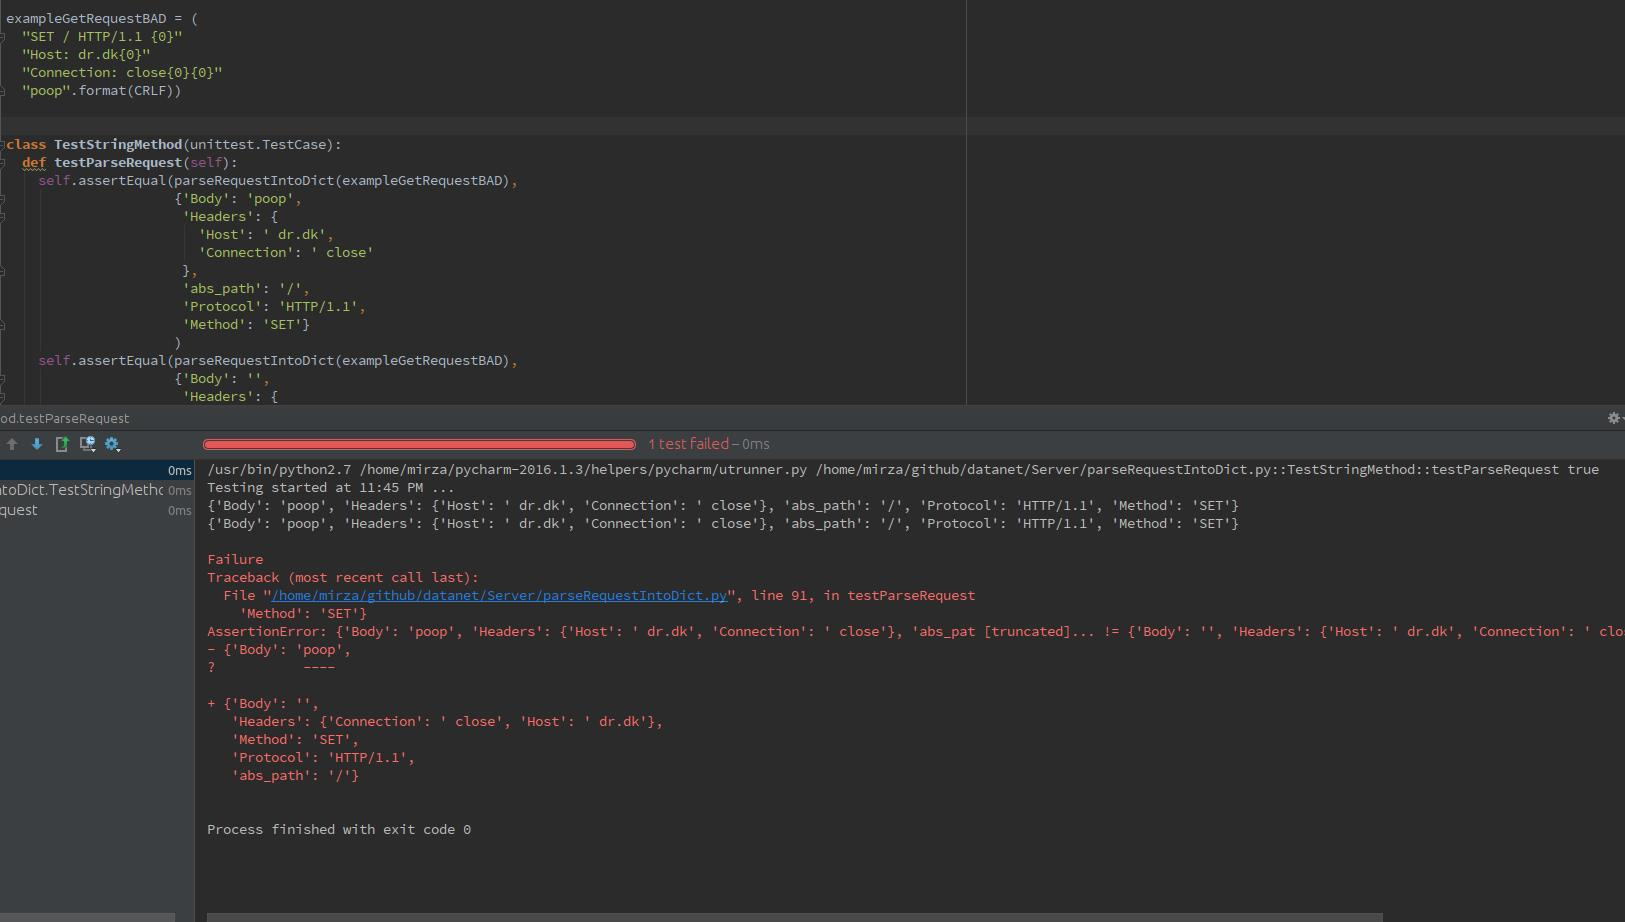
\includegraphics[height=15cm, width=20cm, angle=90]{Screenshot1.jpg}
\newpage
\section{Server with multiple connections}
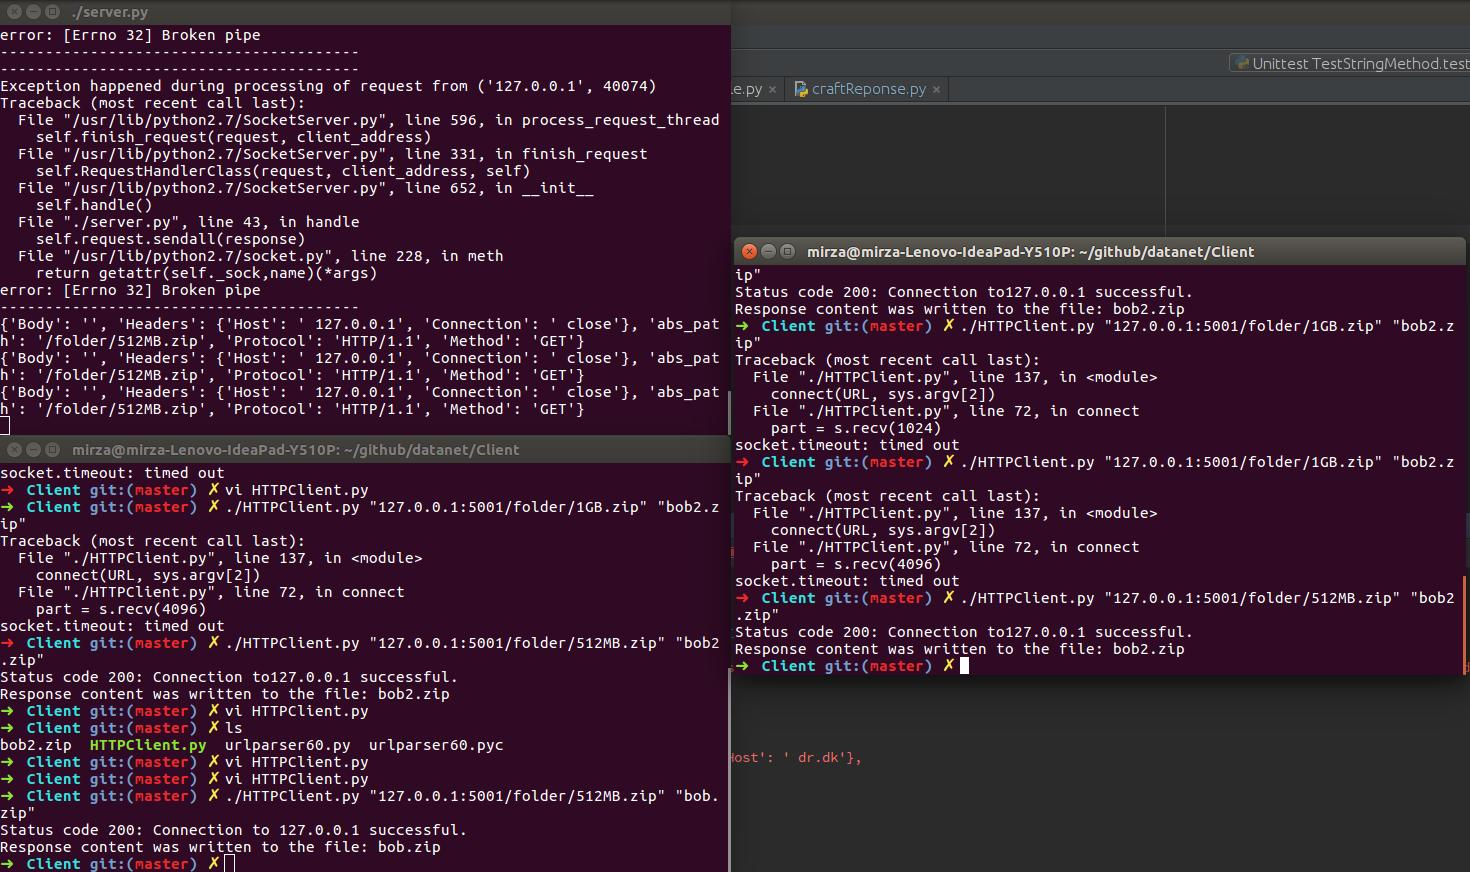
\includegraphics[height=15cm, width=20cm, angle=90]{Screenshot2.jpg}
\newpage
\section{MD5 Sums for the files}
\url{http://www.thinkbroadband.com/download/}\\
5b563100babfef2f2ec9ab2d55e97fd1  100MB.zip\\
3aa55f03c298b83cd7708e90d289afbd  10MB.zip\\
286e80b3b7420263038ab06d76774043  1GB.zip\\
f00be31bb73fe783209497d80aa1de89  1MB.zip\\
3389a0b30e05ef6613ccbdae5d9ec0bd  200MB.zip\\
9017804333c820e3b4249130fc989e00  20MB.zip\\
528972766cd55c26a570829775afd2a8  2MB.zip\\
2699c63cb6699b2272f78989b09e88b1  50MB.zip\\
dfe6504e0e8283357a3443234b266246  512MB.zip\\
b3215c06647bc550406a9c8ccc378756  5MB.zip\\




%\balancecolumns % GM June 2007
% That's all folks!
\end{document}
